\section{Semaine 1 : 06/02/2023 - 10/02/2023}
\graphicspath{{semaines/semaine_1/images/}}

\begin{abstract}
	Pendant cette première semaine, j'ai du me familiariser avec le code "phifem" écrit par Vincent Vigon et les codes de génération des données fournit par Killian. L'idée étant de comprendre comment générer les données avec FEniCS pour ensuite les faire apprendre par un FNO. Après la réunion du 07/02, il semblerait que le sujet du stage porte sur l'entrainement d'un FNO puis la correction/certification des prédictions.
\end{abstract}

\subsection{Génération des données}

Le code fournit par Killian (\href{https://colab.research.google.com/drive/1AJr5JaNs_gnbJce7zE2rfbjicwPxjdtL}{"Data\_Generation\_moving\_ellipse\_poisson"}) a pour but de faire varier la levelset. J'ai donc repris ce code afin de générer dans un premier temps les données solution d'un problème de Poisson avec condition de Dirichlet homogène (\href{https://colab.research.google.com/drive/1dHHFmfDs9XiMoT5EMKXQ1OFFKB3138c2}{"DataGen\_PhiFEM\_f\_gaussienne"}). 

On considère $\Omega$ le cercle de rayon $\sqrt{2}/4$ et de centre $(0.5,0.5)$ avec $\Phi(x,y)=-1/8+(x-1/2)^2+(y-1/2)^2$ et le domaine fictif $O=(0,1)^2$.

On souhaite résoudre 
\begin{equation*}
	\begin{cases}
		-\Delta u &= f\,, \quad \text{dans $\Omega$}\,, \\
		u &= 0\,, \quad \text{sur $\Gamma$}\,, \\
	\end{cases}
\end{equation*}
où 
$$f(x,y) = \exp\left(-\frac{(x-\mu_0)^2 + (y-\mu_1)^2}{2\sigma^2}\right)\,, $$ 
avec $\sigma \sim \mathcal{U}([0.1,0.6])$ et $\mu_0, \mu_1 \sim \mathcal{U}([0.5-\sqrt{2}/4, 0.5+\sqrt{2}/4])$ à condition que $\phi(\mu_0, \mu_1) < -0.05$. 

\begin{minipage}{0.48\linewidth}
	\centering
	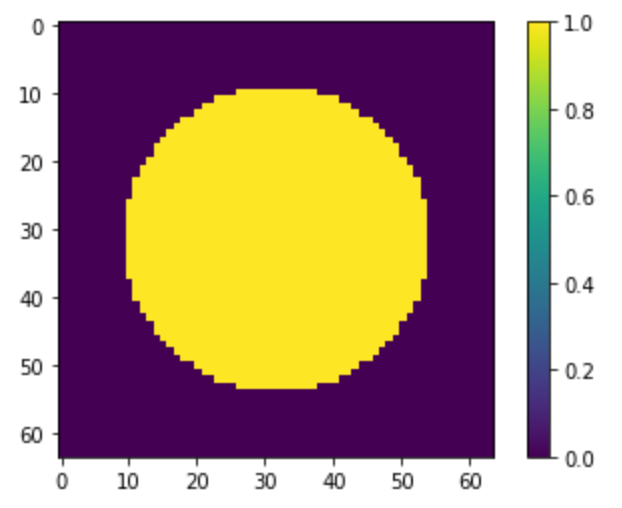
\includegraphics[width=0.5\linewidth]{domaine.png}
\end{minipage}
\begin{minipage}{0.48\linewidth}
	\centering
	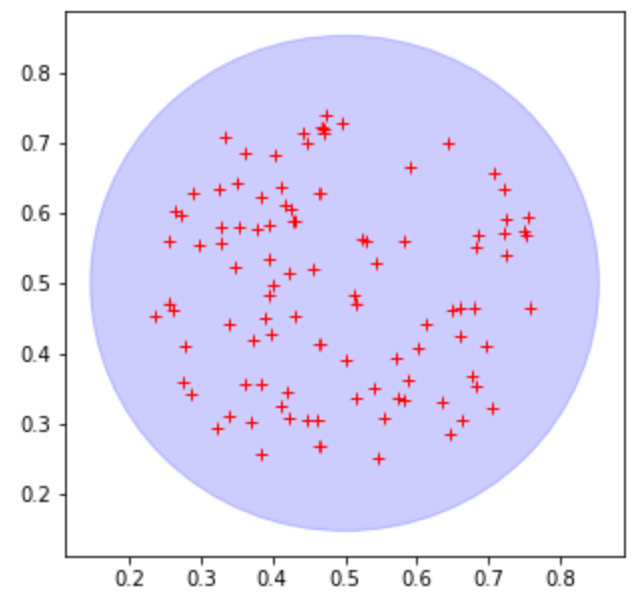
\includegraphics[width=0.45\linewidth]{parametres.png}
\end{minipage}

La fonction \textit{create\_data} renvoie le nombre donné de $F$ et les paramètres associés choisis uniformément. 

\textbf{Formulation faible :}
$$\int_{\Omega_h}\nabla(\bar{\phi}w)\nabla(\bar{\phi}v)-\int_{\partial\Omega_h}\frac{\partial}{\partial n}(\bar{\phi}w)\bar{\phi}v+G_h(w,v)=\int_{\Omega_h}f\bar{\phi}v+G_h^{rhs}(v)$$
avec
$$G_h(w,v)=\sigma h\sum_{E\in\mathcal{F}_h^\Gamma}\int_E\left[\frac{\partial}{\partial n}(\bar{\phi}w)\right]\left[\frac{\partial}{\partial n}(\bar{\phi}v)\right]+\sigma h^2\sum_{T\in\mathcal{T}_h^\Gamma}\int_T \Delta(\bar{\phi}w)\Delta(\bar{\phi}v)$$
et
$$G_h^{rhs}(v)=-\sigma h^2\sum_{T\in\mathcal{T}_h^\Gamma}\int_T f\Delta(\bar{\phi}v)$$

On utilise \href{https://fenicsproject.org/}{FEniCS} (solveur d'EDP) pour résoudre le problème. 

On va finalement stocker les résultats au format npy dans les fichiers "F.npy", "agentParams.npy" et "U.npy"

\newpage

\subsection{FNO}

De la même manière que pour la génération des données, il a fallu reprendre le code de Vincent Vigon (\href{https://colab.research.google.com/drive/1dOIb8N1i6FWXZPOvuP8xFIxmf0kjQysR}{"phifem"}) afin de l'adapter au problème considéré (\href{https://colab.research.google.com/drive/1-OdXA3xj5_X-xwvYplRStopU1yQe7AOg}{phifem\_f\_gaussienne}). 

Une première étape fut donc la lecture d'article sur les FNO (Fourier Neural Operator). Voici un schéma descriptif de ce type de réseau de neurones. 

\begin{minipage}{\linewidth}
	\centering
	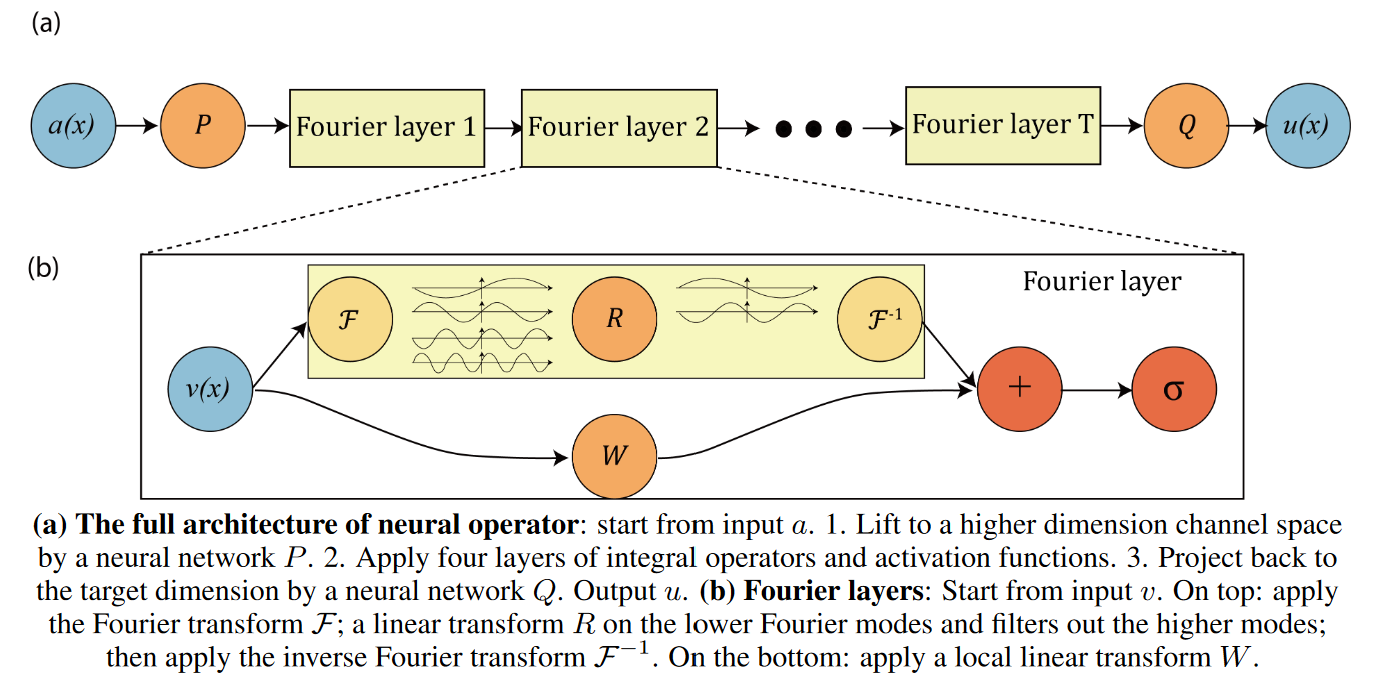
\includegraphics[width=0.7\linewidth]{FNO.png}
\end{minipage}

L'idée étant que le réseau nous retourne $u$.

\begin{Rem}
	ERREUR : il doit nous retourner $w$ car on connait déjà la levelset et pour la correction, ça n'a pas de sens de faire $\phi u=\phi^2 w$.
\end{Rem}

\subsection{Correction}

On veut en fait résoudre le même problème sauf que cette fois-ci, on définit une nouvelle levelset $\bar{\phi}=\phi u$ (où $u$ est la sortie du FNO).

On résout alors le nouveau problème $z=\bar{\phi}C$ :
\begin{equation*}
	\begin{cases}
		-\Delta z &= f\,, \quad \text{dans $\Omega$}\,, \\
		z &= 0\,, \quad \text{sur $\Gamma$}\,, \\
	\end{cases}
\end{equation*}

\begin{Rem}
	L'idée étant d'appliquer la correction sur un millage plus grossier que le réseau. Ainsi FNO+Corr plus précis que Phifem classique et plus rapide.
\end{Rem}

Les résultats obtenus (en prenant ici $u_{ex}=cos\left(\frac{\pi}{2}\times\left(\frac{4}{\sqrt{2}}\right)^2\times\left((x-0.5)^2+(y-0.5)^2\right)\right)$) ne sont pas bons :

\begin{minipage}{\linewidth}
	\centering
	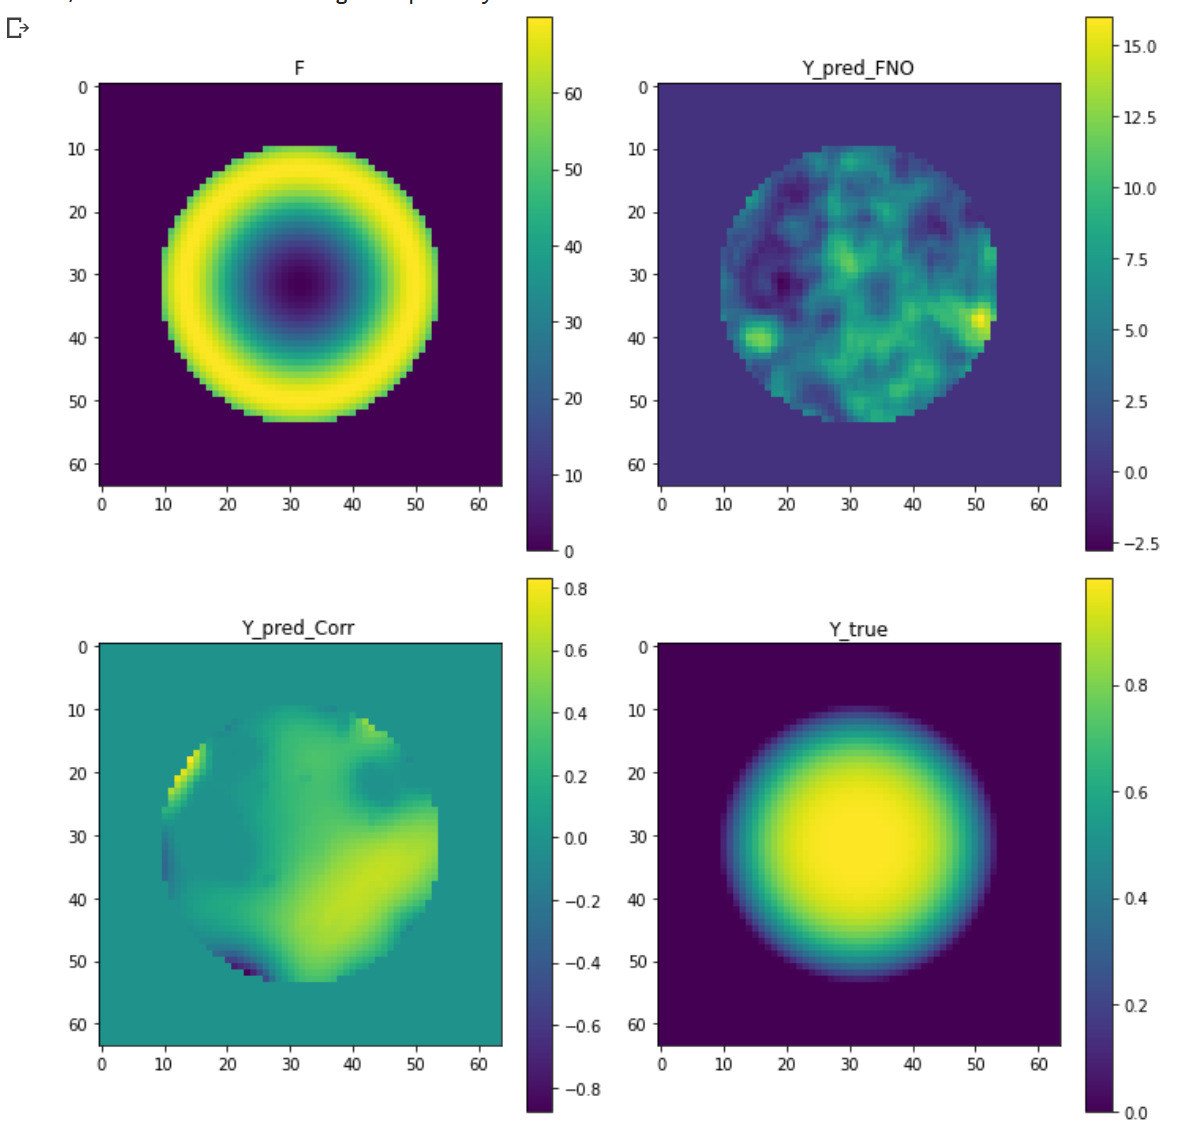
\includegraphics[width=0.45\linewidth]{resultats.png}
\end{minipage}

\begin{Rem}
	ERREUR : C'est logique !!! Le réseau n'a pas été entrainé pour ça ! (+ pb remarque d'avant.)
\end{Rem}



